\documentclass[twocolumn]{IEEEtran}
\usepackage{graphicx}
\usepackage[utf8x]{inputenc}
\usepackage{times}
\usepackage{amssymb,amsfonts}
\usepackage{pict2e}
\usepackage{float}
\usepackage[all]{xy}
\usepackage{graphics,graphicx,color,colortbl}
\usepackage{subfigure}
\usepackage{wrapfig}
\usepackage{multicol}
\usepackage{cite}
\usepackage{url}
\usepackage[tbtags]{amsmath}
\usepackage{amsmath,amssymb,amsfonts,amsbsy}
\usepackage{bm}
\usepackage{listings}
\usepackage{algorithm}
\usepackage{algorithmic}
\usepackage[centerlast, small]{caption}
\usepackage[colorlinks=true, citecolor=blue, linkcolor=blue, urlcolor=blue, breaklinks=true]{hyperref}
\hyphenation{ele-men-tos he-rra-mi-en-ta cons-tru-yen trans-fe-ren-ci-a pro-pu-es-tas si-mu-lar}

\begin{document}
\title{Control PID}
\author{Israel Ricardo Bernal Sánchez Código: $261613$\\
	Felipe Castañeda Prieto Código $285728$\\
	David Ricardo Martínez Hernández Código: $261931$\\
	Oscar Andrés Urbano Vallejo Código: $261683$}
\maketitle
\markboth{Universidad Nacional de Colombia}{}
\floatname{algorithm}{Algoritmo}

\begin{abstract}
 En el siguiente informe se implementaron varias configuraciones con diferentes métodos de sintonización entre ellos se encuentran: El Método de cancelación de polo-cero, Método de Ubicación de polos, Método del Lugar geométrico de las Raíces, sintonización Ziegler \& Nichols y criterios IAE e ITAE. Simulándolos en Matlab e implementados por medio del BricxCC, obteniendo una comparación teórico-práctica, y así tomando una comparación  más precisa y aproximada a la realidad.
\end{abstract}

\begin{keywords}
 Control P PI PD y PID, Controladores, Error Permanente, Método de cancelación de polo-cero, Método de Ubicación de polos, Método del Lugar geométrico de las Raíces, Sintonización, Sobrenivel Porcentual, Tiempo de estabilización.
\end{keywords}

\section{Introducción}
\noindent
En esta práctica de laboratorio se desarrollaron diferentes tipos de controladores para una planta determinada, observando y analizando las diferentes acciones del control P, I y D, en su parte dinámica y su parte estática, aplicando diferentes técnicas de sintonización como Ziegler \& Nichols y criterios IAE e ITAE, También utilizando el método de cancelación de polo-cero, Método de Ubicación de polos, Método del Lugar geométrico de las Raíces, para cumplir diferentes requerimientos como  Sintonización, Sobrenivel Porcentual, Tiempo de estabilización y Error Permanente.\\

\section{Procedimiento}
\noindent
La prática está divida en dos partes: Métodos Clásicos de Sintonización PID, y Control PID por Síntesis, Cancelación Polo-Cero y LGR.

\subsection{Métodos Clásicos de Sintonización PID}
\noindent

\subsubsection{Punto 4.1.1 y 4.1.2}
\noindent
\begin{figure}[H]
	\centering
		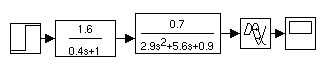
\includegraphics[scale=1]{tf1.png}
	\caption{Diagrama de bloques del sistema intercambiador de calor en lazo abierto}
	\label{fig1}
\end{figure}
\noindent
El sistema en lazo abierto presenta el siguiente comportamiento frente a una entrada tipo escalón de magnitud $1$:
\begin{figure}[H]
	\centering
		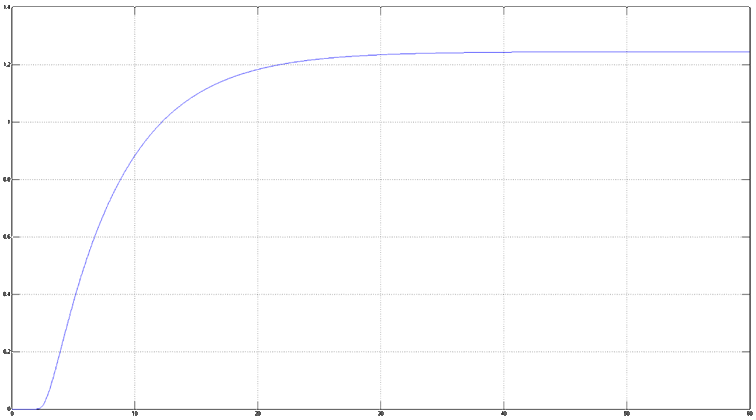
\includegraphics[scale=0.35]{simulation11.png}
	\caption{Diagrama de bloques del sistema intercambiador de calor en lazo abierto}
	\label{fig12}
\end{figure}
\noindent
El comportamiento del sistema intercambiador de calor en lazo abierto puede ser aproximado a un sistema de primer orden más tiempo muerto, que produzca un comportamiento similar al de la planta original y tenga la siguiente función de transferencia:
\begin{equation}
 G\left( s \right) = \frac{K}{{\tau s + 1}}e^{ - t_0 s} 
\label{ecu101}
\end{equation}
\noindent
Se observa que el comportamiento de la planta en lazo abierto tiene un error de posición diferente de cero  al estabilizarse en un valor diferente a la amplitud del paso de entrada por lo que:
\begin{equation}
 K = \frac{{\Delta _{OutPut} }}{{\Delta _{InPut} }} = \frac{{1.244}}{1} = 1.244
\label{ecu102}
\end{equation}
\noindent
La respuesta del sistema en lazo abierto presenta una demora al inicio debió al delay del sistema y a su naturaleza de tercer orden que hace que presente la curvatura al comienzo de la respuesta, lo que es representado en la aproximación como el tiempo muerto. El cálculo del tiempo de establecimiento y el tiempo muerto se realiza de la siguiente forma:
\begin{itemize}
 \item Se ubican los puntos $t_1  = \left( {t_0  + \frac{\tau }{s}} \right)$ y $t_2  = \left( {t_0  + \tau} \right)$, donde $t_0$ es el tiempo muerto, a partir de:\\
$\Delta y\left( {t_0  + \tau } \right) = 0.632\Delta y_{ss}$ y $\Delta y\left( {t_0  + \frac{\tau }{s}} \right) = 0.283\Delta y_{ss}$\\
Donde a $0.632\Delta =0.7862$, le corresponde el tiempo $t_2=8.66\ \ s$
Donde a $0.283\Delta =0.3521$, le corresponde el tiempo $t_1=4.88\ \ s$
 \item A partir de los datos anteriores se calculan los siguientes valores:\\
$$\tau  = \frac{3}{2}\left( {t_2  - t_1 } \right) = \frac{3}{2}\left( {8.66 - 4.88} \right) = 5.67\ \ s$$
$$t_0  = 8.66 - 5.67 = 2.99\ \ s$$
\end{itemize}
\noindent
La función de transferencia correspondiente es:
\begin{equation}
 G_{2}\left( s \right) = \frac{{1.244}}{{5.67s + 1}}e^{ - 2.99s}
\label{ecu103}
\end{equation}
\noindent
El siguiente diagrama de bloques presenta la simulación del sistema de primer orden encontrado en comparación del sistema intercambiador de calor original:
\begin{figure}[H]
	\centering
		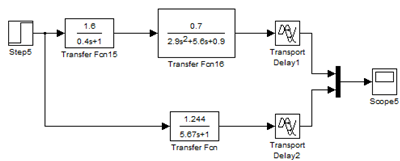
\includegraphics[scale=0.5]{block.png}
	\caption{Diagrama de bloques del sistema intercambiador de calor y el modelo FOPDT}
	\label{fig13}
\end{figure}
\noindent
La siguiente figura muestra la respuesta de la función $G_2$, y como es su comportamiento respecto la función anterior:
\begin{figure}[H]
	\centering
		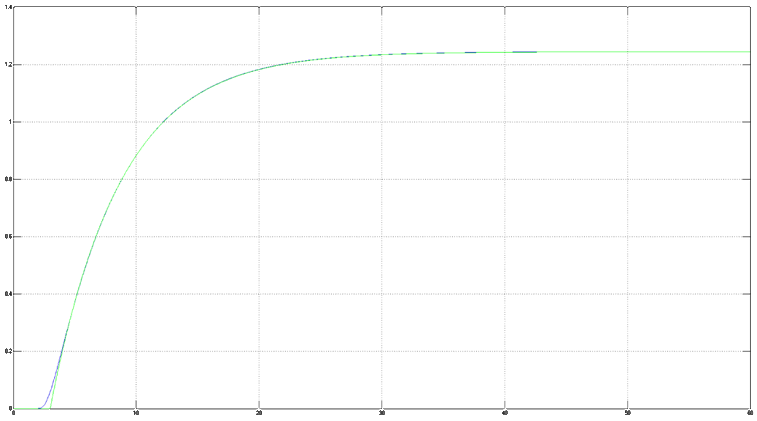
\includegraphics[scale=0.3]{simulation12.png}
	\caption{Respuesta del modelo FOPDT del sistema intercambiador de calor}
	\label{fig14}
\end{figure}

\subsubsection{Punto 4.1.3}
\noindent
\begin{figure}[H]
	\centering
		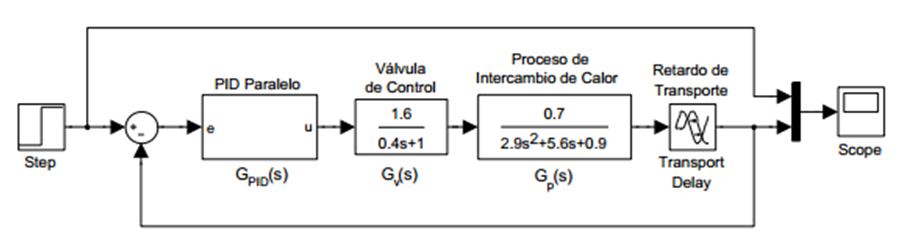
\includegraphics[scale=0.27]{tf13.png}
	\caption{Diagrama de bloques para el intercambiador de calor con un control PID paralelo}
	\label{fig16}
\end{figure}
\noindent
A través del sistema mostrado en la Fig. \ref{fig16}, se realiza la implementación del compensador PID al sistema de intercambio de calor y se varían los parámetros P. I, y D. 
\begin{figure}[H]
	\centering
		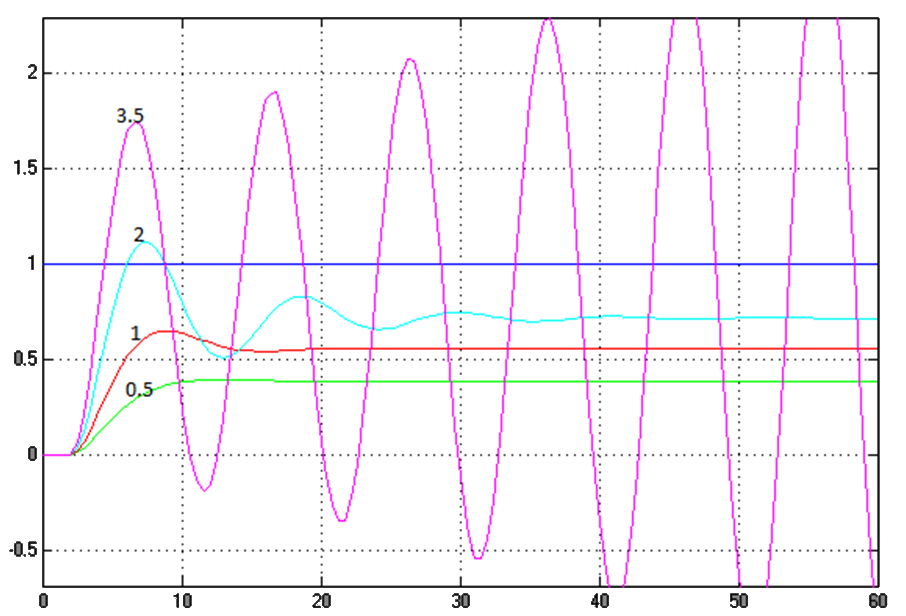
\includegraphics[scale=0.27]{kvariante.png}
	\caption{Variaciones de $K_c$ compensador PID.}
	\label{fig17}
\end{figure}
\noindent
Al aumentar el valor de $K_c$ (con las partes derivativa e integral desconectadas) del compensador PID se observa que mejora la ganancia y el sistema responde más rápido, esto a costo de la estabilidad, para valores muy grandes de $K_c$ el sistema se vuelve altamente inestable, esto se observa claramente cuando $K_c=3.5$ , en esta parte es claro que para que la respuesta sea buena hace falta una corrección de el error de estado estacionario (parte Integral del controlador).
\begin{figure}[H]
	\centering
		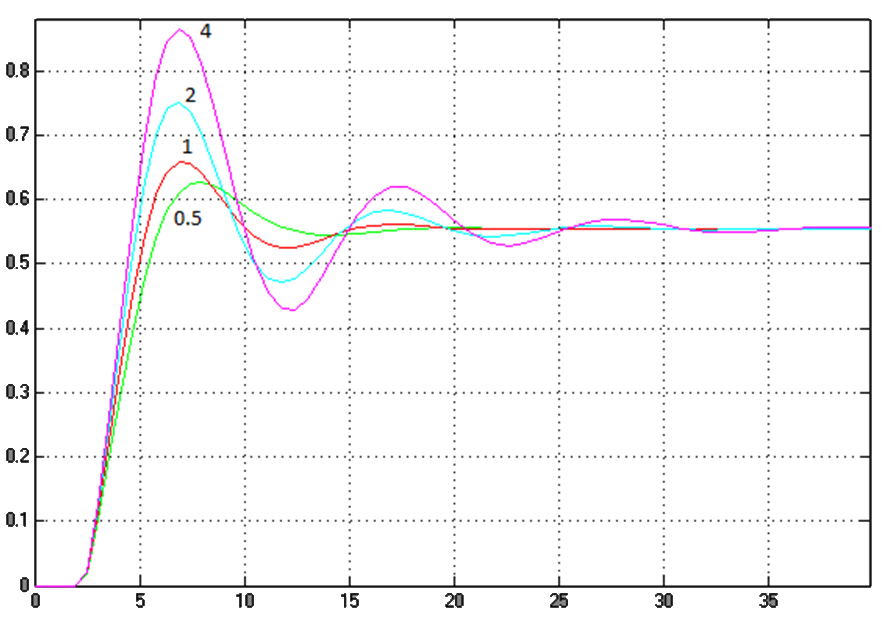
\includegraphics[scale=0.27]{tdvariacion.png}
	\caption{Variación de $T_d$ compensador PID.}
	\label{fig18}
\end{figure}
\noindent
En laFig. \ref{fig18} se evidencia como a través del aumento de $T_d$ el sistema responde mucho más rápido, sin embargo dicho aumento produce también un sobrepico muy grande, además de que no se corrige el error de estado estacionario (tarea de la parte Integral del controlador), finalmente se concluye que el parámetro $T_d$ solo afecta en la velocidad de respuesta del sistema y su sobrepico incial.
\begin{figure}[H]
	\centering
		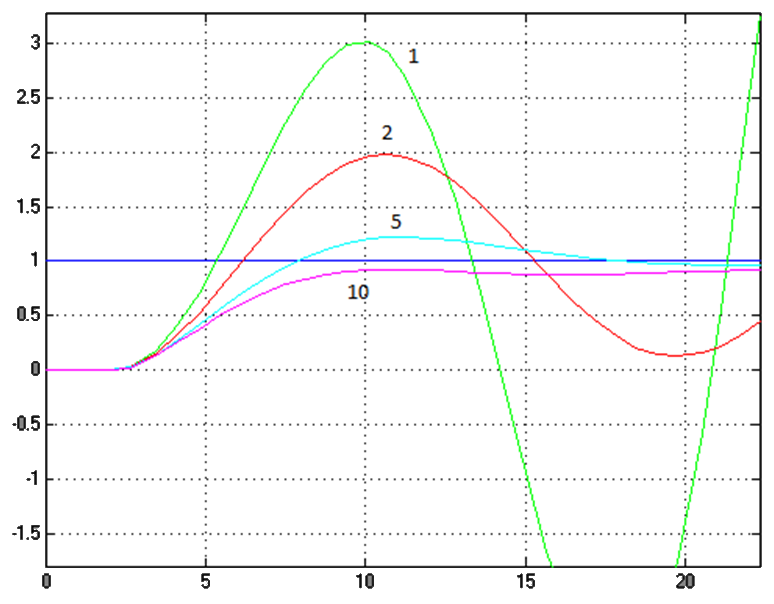
\includegraphics[scale=0.27]{tivariacion.png}
	\caption{Variación de $T_i$ compensador PID.}
	\label{fig19}
\end{figure}
\noindent
Como se observa de la Fig. \ref{fig19} el parámetro Ti afecta la respuesta en estado estacionario del sistema, para valores grandes de este el sistema corrige su error de estado estacionario, sin embargo en valores muy pequeños el sistema se vuelve altamente inestable. La clave en la elección de este parámetro esta en encontrar el balance perfecto entre tiempo de estabilización y un sobrepico adecuado a cada aplicación.\\
Finalmente se concluye que la respuesta del sistema se puede optimizar utilizando una combinación adecuada de estos tres parámetros ($K_c$, $T_i$ ,$T_d$).

\subsubsection{Punto 4.1.4}
\noindent
\begin{figure}[H]
	\centering
		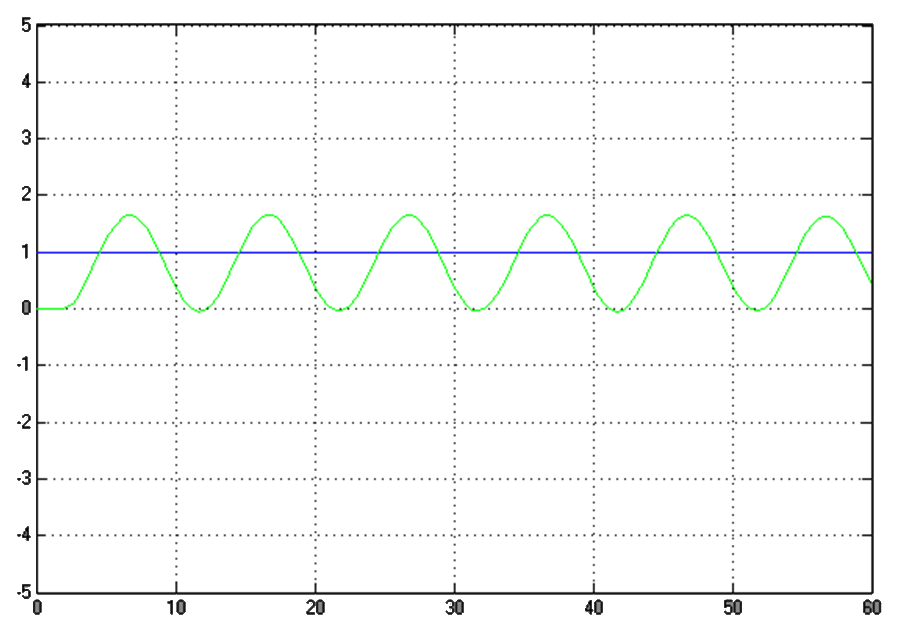
\includegraphics[scale=0.27]{sumilation20.png}
	\caption{Oscilación permanente en $K_c= 3.275$.}
	\label{fig30}
\end{figure}
\noindent
Se desconectaron la parte integral y derivativa del controlador y se varió el $K_c$ de dicho controlador, finalmente se obtuvo una respuesta con una oscilación permanente para un $kc=3.275=ku$ para este el periodo de oscilación ultima es $Tu= 10$, a través de estos dos valores y ayudados de la TABLA \ref{tab1} se determinaron los demás valores para el respectivo  controlador  PI y PID.
\begin{table}[H]
	\centering
\begin{tabular}{|c|c|c|c|}\hline
Compensador & $K'_c$ & $T'_i$ & $T'_d$ \\ \hline
$P$ & $\frac{K_u}{2}$ & $---$ & $---$ \\ \hline
$PI$ & $\frac{K_u}{2.2}$ & $\frac{T_u}{1.2}$ & $---$ \\ \hline
$PID$ & $\frac{K_u}{1.7}$ & $\frac{T_u}{2}$ & $\frac{T_u}{8}$ \\ \hline
    \end{tabular}
	\caption{Tabla sintonización ganancia última.}
	\label{tab1}
\end{table}
\begin{table}[H]
	\centering
\begin{tabular}{|c|c|}\hline
De PID Paralelo a PID serie & De PID serie a PID paralelo \\ \hline
$K'_c  = 0.5 + \sqrt {0.25 - \frac{{T_d }}{{T_i }}}$ & $K_c  = K'_c \left( {1 + \frac{{T'_d }}{{T'_i }}} \right)$ \\ \hline
$T'_i  = T_i \left( {0.5 + \sqrt {0.25 - \frac{{T_d }}{{T_i }}} } \right)$ & $T_i=T'_i+T'_d$ \\ \hline
$T'_d  = \frac{{T_d }}{{0.5 + \sqrt {0.25 - \frac{{T_d }}{{T_i }}} }}$ & $T_d  = \frac{{T'_i T'_d }}{{T'_i  + T'_d }}$ \\ \hline
    \end{tabular}
	\caption{Conversión Serie-Paraleo.}
	\label{tab2}
\end{table}
\noindent
Para el controlador PI se tiene:\\
$K_u = 3.275$, $T_u=10seg$, $K'_c= \frac{K_u}{2.2}=1.4886$, $T'_i=\frac{T_u}{1.2}=8.333$.\\
Estos parámetros son los mismos en configuración paralelo debido a la ausencia de $T'_d$.\\
Con la sintonización de estos parámetros se procede a realizar la correspondiente simulación:
\begin{figure}[H]
	\centering
		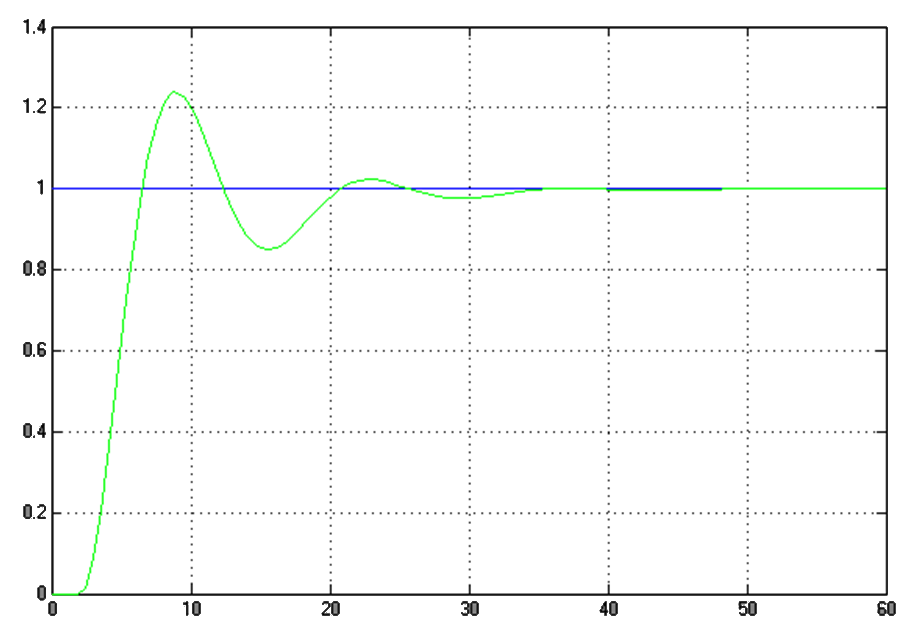
\includegraphics[scale=0.27]{figura1.png}
	\caption{Sintonización PI método de ganancia última.}
	\label{fig31}
\end{figure}
\noindent
\textbf{Controlador PID}\\
$K_u= 3.275$, $T_u=10s$, $K'_c= \frac{K_u}{1.7} =  1.9264$, $T'_i = \frac{Tu}{2} =  5$, $T'_d = \frac{Tu}{8} =  1.25$. Para estos parámetros se hace la correspondiente transición a paralelo haciendo uso de la TABLA \ref{tab2}. Se obtiene
$$K_c=  K'_c+ K'_c\frac{T'_d}{T'_i}= 1.9264+  1.9264\frac{1.25}{5}= 2.408$$
$$T_i= T'_i + T'_d = 5 + 1.25 = 6.25$$
$$T_d= \frac{T'_iT'_d}{T'_i + T'_d} = \frac{5*1.25}{5+1.25}= 1 $$
Con la sintonización de estos parámetros se procede a realizar la correspondiente simulación:
\begin{figure}[H]
	\centering
		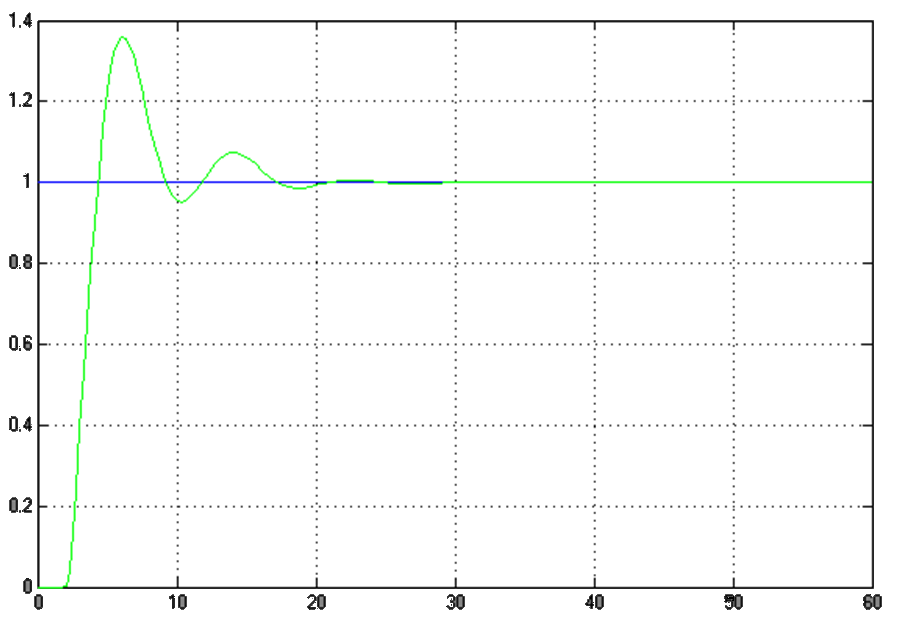
\includegraphics[scale=0.27]{figura2.png}
	\caption{Sintonización PID método de ganancia ultima.}
	\label{fig32}
\end{figure}
\noindent
Como se observa en la Fig. \ref{fig32} la sintonización PI es bastante buena el sobrepico no es muy grande ($M_p(\%)= 22 (\%)$) y el sistema se estabiliza rápidamente (aproximadamente $18$ segundos). Caso contrario en la sintonización PID el sobrepico es considerablemente grande ($M_p (\%)=38\%$ aproximadamente), aunque el sistema responde mucho más rápido se estabiliza prácticamente al mismo tiempo que el PI.\\
Finalmente se concluye que la mejor sintonización para este controlador es el obtenido en la parte PI.

\subsubsection{Punto 4.1.5}
\noindent
\begin{table}[H]
	\centering
\begin{tabular}{|c|c|c|c|}\hline
Compensador & $K'_c$ & $T'_i$ & $T'_d$ \\ \hline
$P$ & $\frac{1}{K}\left( {\frac{{t_0 }}{\tau }} \right)^{ - 1} $ & $---$ & $---$ \\ \hline
$PI$ & $\frac{0.9}{K}\left( {\frac{{t_0 }}{\tau }} \right)^{ - 1} $ & $3.33t_0$ & $---$ \\ \hline
$PID$ & $\frac{1.2}{K}\left( {\frac{{t_0 }}{\tau }} \right)^{ - 1} $ & $2.0t_0$ & $0.5t_0$ \\ \hline
    \end{tabular}
	\caption{Sintonización por medio de FOPDT.}
	\label{tab3}
\end{table}
\noindent
En el punto 4.1.2 ya se calculo el modelo de primer orden con retraso.
\begin{equation}
 G\left( s \right) = \frac{K}{{\tau s + 1}}e^{ - t_0 s};\ \ G\left( s \right) = \frac{{1.244}}{{5.67s + 1}}e^{ - 2.99s} 
\label{ecu000}
\end{equation}
\begin{equation}
 K=1.244,\ \ t_0 = 2.99s,\ \ \tau=5.67s
\label{ecu001}
\end{equation}
\noindent
Con estos valores y haciendo uso de la tabla 3 se determinan los valores $K'_c$, $T'_i$ y $T'_d$, posteriormente se les realiza su respectiva conversión serie–paralelo y se simulan:\\
\textbf{Controlador PI}\\
$K'_c=1.3719$, $T'_i=9.9567$.\\
Estos parámetros son los mismos en configuración paralelo debido a la ausencia de $T'_d$. Con la sintonización de estos parámetros se procede a realizar la correspondiente simulación:
\begin{figure}[H]
	\centering
		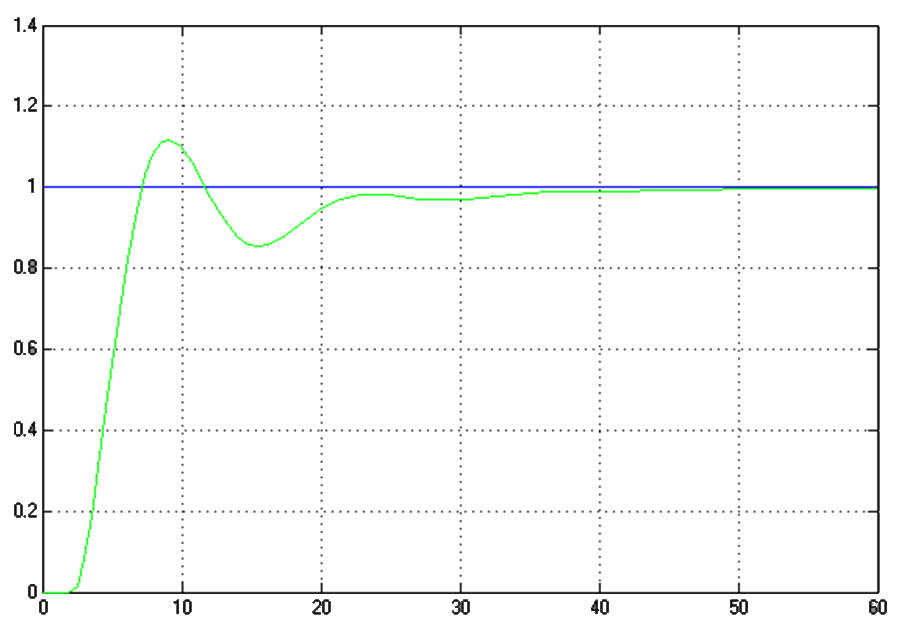
\includegraphics[scale=0.28]{3.png}
	\caption{Sintonización PI método FOPDT.}
	\label{fig003}
\end{figure}
\noindent
\textbf{Controlador PID}\\
$K'_c=1.8292$, $T'_i=5.98$, $T'_d=1.495$\\
Para estos parámetros se hace la correspondiente transición a paralelo haciendo uso de la TABLA \ref{tab2}.\\
$K_c=2.2865$, $T_i=7.475$, $T_d=1.169$\\
Con la sintonización de estos parámetros se procede a realizar la correspondiente simulación:
\begin{figure}[H]
	\centering
		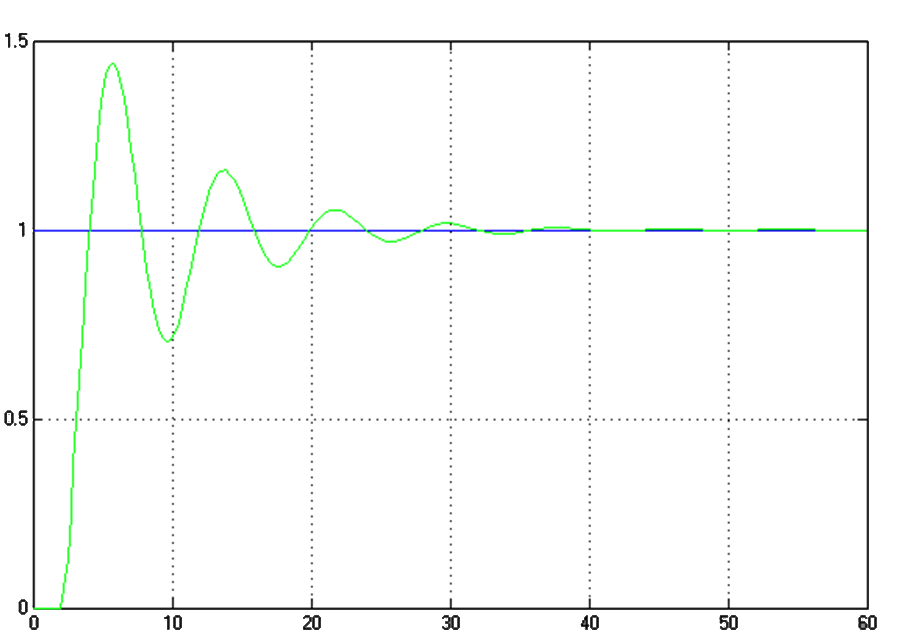
\includegraphics[scale=0.25]{4.png}
	\caption{Sintonización PID método FOPDT.}
	\label{fig004}
\end{figure}
\noindent
Por medio de este método (FOPDT) la sintonización PI es bastante buena, presenta un $M_P(\%)= 11\%$ y se estabiliza aproximadamente un poco después de  los $20$ segundos, por otro lado el PID tiene un sobrepico mucho mas grande ($M_P(\%)= 45\%$ aproximadamente) y aunque responde más rápido se demora prácticamente lo mismo que el PI para estabilizarse.\\
Finalmente se concluye que al igual que en el anterior método la mejor sintonización para este controlador es la obtenida en la parte PI.

\subsubsection{Punto 4.1.6}
\noindent
Para la realización de la sintonización por medio de estos dos criterios, se hace uso del modelo de primer orden más tiempo muerto calculado en el punto 4.1.2:
\begin{equation}
 G\left( s \right) = \frac{K}{{\tau s + 1}}e^{ - t_0 s};\ \ G\left( s \right) = \frac{{1.244}}{{5.67s + 1}}e^{ - 2.99s} 
\label{ecu120}
\end{equation}
\begin{equation}
 K=1.244,\ \ t_0 = 2.99s,\ \ \tau=5.67s
\label{ecu121}
\end{equation}
\noindent
Luego por medio de las TABLA \ref{tab4} y TABLA \ref{tab5} se realiza la sintonización PI y PID respectivamente:
\begin{table}[H]
	\centering
\begin{tabular}{|c|c|c|}\hline
\textbf{Parámetros PI} & \textbf{IAE} & \textbf{ITAE} \\ \hline
$K_c=\frac{{a_1 }}{K}\left( {\frac{{t_0 }}{\tau }} \right)^{b_1 }$ & $a_1=0.758$, $b_1=-0.861$ & $a_1=0.586$, $b_1=-0.916$ \\ \hline
$T_i  = \frac{\tau }{{a_2  + b_2 \left( {\frac{{t0}}{\tau }} \right)}}$ & $a_2=1.02$, $b_2=-0.323$ & $a_2=1.03$, $b_2=-0.165$ \\ \hline
    \end{tabular}
	\caption{Sintonización PI métodos IAE – ITAE.}
	\label{tab4}
\end{table}
\noindent
\textbf{IAE}\\
$K_c=1.0571$, $T_i=6.6731$\\
\textbf{ITAE}\\
$K_c=0.8465$, $T_i=6.0128$\\
Con estos parámetros determinados se realiza la simulación para la sintonización PI:
\begin{figure}[H]
	\centering
		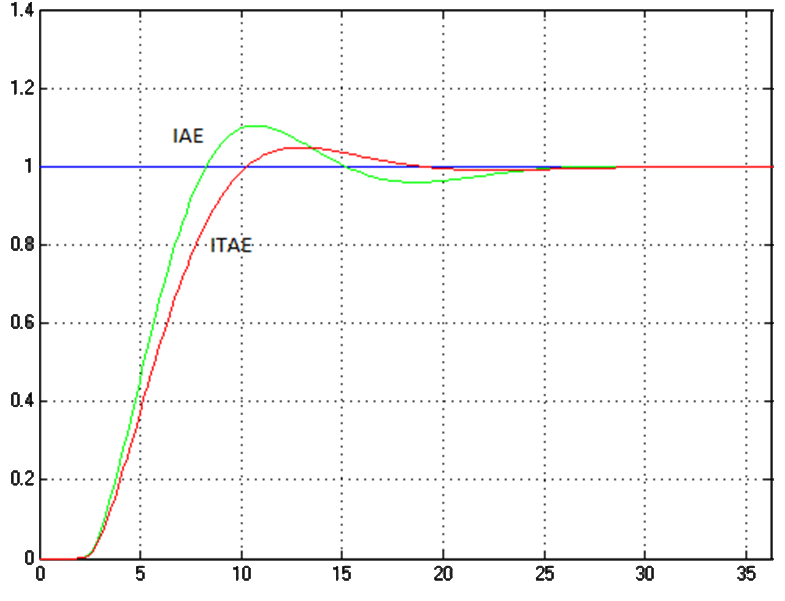
\includegraphics[scale=0.28]{1.png}
	\caption{Sintonización PI criterio IAE – ITAE.}
	\label{fig001}
\end{figure}
\noindent
\textbf{Sintonización PID}
\begin{table}[H]
	\centering
\begin{tabular}{|c|c|c|}\hline
\textbf{Parámetros PID} & \textbf{IAE} & \textbf{ITAE} \\ \hline
$K_c=\frac{{a_1 }}{K}\left( {\frac{{t_0 }}{\tau }} \right)^{b_1 }$ & $a_1=1.086$, $b_1=-0.869$ & $a_1=0.965$, $b_1=-0.855$ \\ \hline
$T_i  = \frac{\tau }{{a_2  + b_2 \left( {\frac{{t0}}{\tau }} \right)}}$ & $a_2=0.74$, $b_2=-0.13$ & $a_2=0.796$, $b_2=-0.147$ \\ \hline
$T_d  = a_3 \tau \left( {\frac{{t_0 }}{\tau }} \right)^{b_3 } $ & $a_3=0.348$, $b_3=0.914$ & $a_3=0.308$, $b_3=0.9292$ \\ \hline
    \end{tabular}
	\caption{Sintonización PID métodos IAE – ITAE.}
	\label{tab5}
\end{table}
\noindent
\textbf{IAE}\\
$K_c=1.5223$, $8.4445$ y $1.0994$\\
\textbf{ITAE}\\
$K_c=1.3407$, $7.8916$ y $2.8595$\\
Con estos parámetros determinados se realiza la simulación para la sintonización PID:
\begin{figure}[H]
	\centering
		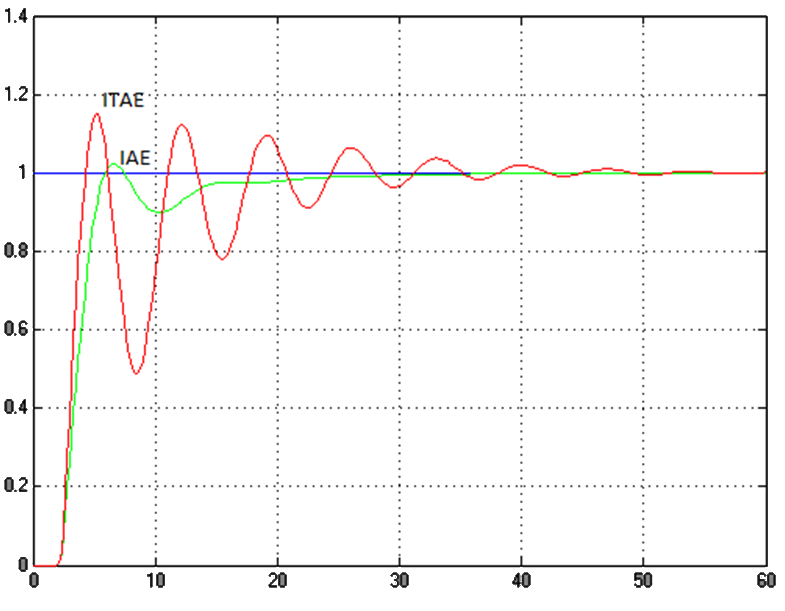
\includegraphics[scale=0.28]{2.png}
	\caption{Sintonización PID criterio IAE – ITAE.}
	\label{fig002}
\end{figure}
\noindent
De los resultados observados en las Fig. \ref{fig001} y \ref{fig002} se concluye que el mejor método de sintonización es el PI con el criterio IAE ya que cumple el mejor balance entre velocidad de respuesta y mínimo sobrepico, además de contar con un tiempo de estabilización mucho mejor el de  los otros.

\subsubsection{Punto 4.1.7}
\noindent
Todos los diferentes métodos y criterios de sintonización presentan fuertes diferencias en su respuesta, esta respuesta esta caracterizada por fuertes oscilaciones  en los sintonizadores PID, esto se debe  al valor del alfa  considerado en todos los sistemas (alfa del tiempo derivativo = $0.125$). Por otra parte se observa que los sistemas de ganancia ultima tienen un tiempo de respuesta muy corto sin embargo están acompañados por fuertes sobrepicos, la respuesta del modelo $FOPDT$  PI esta caracterizada por un buen tiempo de respuesta y un bajo sobrepico sin embargo al aumentarle su parte derivativa PID se vuelve muy inestable. Lo mismo sucede con los sistemas desarrollados por sintonización en base a los criterios \textbf{IAE} e \textbf{ITAE},  presentan respuestas optimas cuando la parte derivativa es anulada. Finalmente se concluye que la mejor respuesta ha sido la generado por el criterio \textbf{IAE} para el controlador PI ya que esta tiene el mejor balance entre tiempo de respuesta y máximo sobrepico, a demás de que su tiempo de estabilización es mucho mejor que el de la mayoría.

\subsection{Control PID por Síntesis, Cancelación Polo-Cero y LGR}
\noindent

\subsubsection{Punto 4.2.1}
\noindent
Al realizar una prueba escalón de magnitud $100\ \ rad/s$ al motor LEGO, se obtienen los siguientes datos experimentales, donde se observa el comportamiento de la velocidad del motor respecto al tiempo.
\begin{figure}[H]
	\centering
		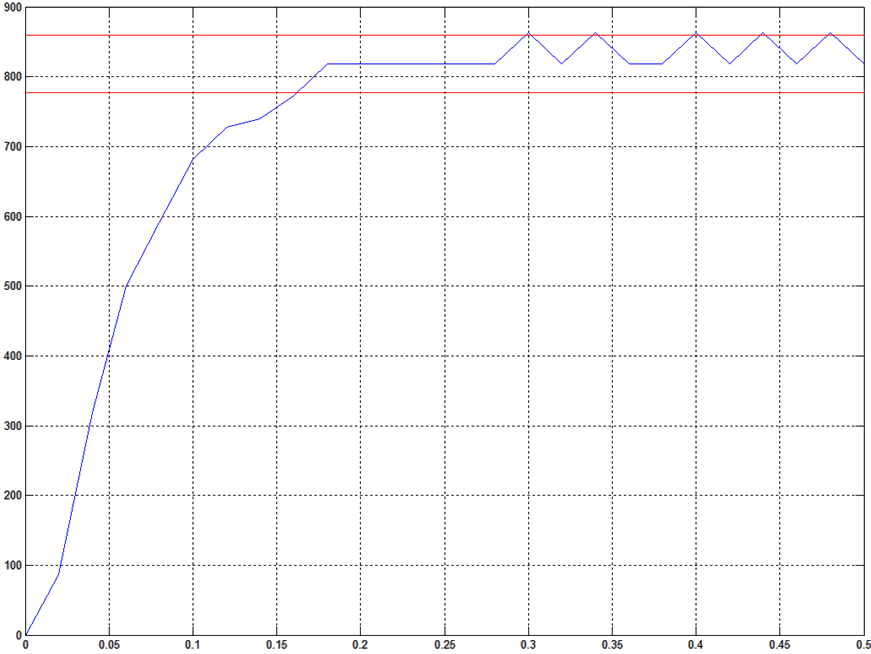
\includegraphics[scale=0.27]{simulation1.png}
	\caption{Velocidad (rad/s) vs tiempo (s) del motor LEGO}
	\label{fig4}
\end{figure}
\noindent
La respuesta encontrada muestra una dinámica de primer orden, y a partir de una aproximación del 5\% se representa el funcionamiento del motor por medio de la siguiente función de transferencia
\begin{equation}
 G\left( s \right) = \frac{{8.181818}}{{0.054s + 1}}
\label{ecu7}
\end{equation}
\noindent
La función de transferencia $G(s)$ es de primer orden sin tiempo muerto, y se toma como base para los puntos posteriores.

\subsubsection{Punto 4.2.2}
\noindent
Debido a que la planta es de primer orden y se desea realizar el control PI, el sistema en lazo cerrado muestra una dinámica de segundo orden, lo que permite aproximar los parámetros de $\zeta$ y $\omega _n$ para cumplir con las especificaciones determinadas. Gracias a que se realiza un control de tipo integral, el sistema es de tipo uno, por lo que el error permanente de posición es cero.
Se establece un sobre nivel porcentual de 6\% para el funcionamiento del sistema.
\begin{figure}[H]
	\centering
		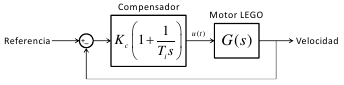
\includegraphics[scale=1]{tf2.png}
	\caption{Sistema de control de velocidad con compensador PI}
	\label{fig2}
\end{figure}
\noindent
Donde:
\begin{equation}
 G\left( s \right) = \frac{{K_p }}{{\tau s + 1}}
\label{ecu100}
\end{equation}
\noindent
La planta de lazo cerrado quedaría de la siguiente manera:
\begin{equation}
 G_{LC} \left( s \right) = \frac{{K_p K_c \left( {T_i s + 1} \right)}}{{K_p K_c \left( {T_i s + 1} \right) + T_i s\left( {\tau s + 1} \right)}}
\label{ecu1}
\end{equation}
\begin{equation}
 G_{LC} \left( s \right) = \frac{{\frac{{K_p K_c \left( {T_i s + 1} \right)}}{{T_i \tau }}}}{{s2 + \frac{{K_p K_c T_i  + T_i }}{{T_i \tau }}s + \frac{{K_p K_c }}{{T_i \tau }}}}
\label{ecu2}
\end{equation}
\noindent
Comparado con la función de transferencia de segundo orden obtenemos:
\begin{equation}
 2\zeta \omega _n  = \frac{{K_p K_c  + 1}}{\tau } ;\ \ \omega _n ^2  = \frac{{K_p K_c }}{{T_i \tau }}
\label{ecu3}
\end{equation}
\noindent
Para el máximo sobre pico se tiene que es
\begin{equation}
 Mp\left( \%  \right) = e^{\frac{{ - \pi \zeta }}{{\sqrt {1 - } \zeta }}} 
\label{ecu5}
\end{equation}
\noindent
Para el tiempo de establecimiento se utilizó la siguiente ecuación
\begin{equation}
 t_p = \frac{3}{\zeta \omega _n} \Longrightarrow \omega _n= \frac{3}{t_p \zeta}
\label{ecu4}
\end{equation}
\noindent
Dado que el $\tau$, $t_p$ y $K_p$ son conocidos se puede determinar los valores de $T_i$ y de $K_c$.
Los resultados obtenidos al hacer el despeje matemático fueron:
\begin{equation}
 K_c=-0.043022893831215\ \ y \ \ T_i=-0.0823
\label{ecu6}
\end{equation}
\noindent
la simulación obtenida fue
\begin{figure}[H]
	\centering
		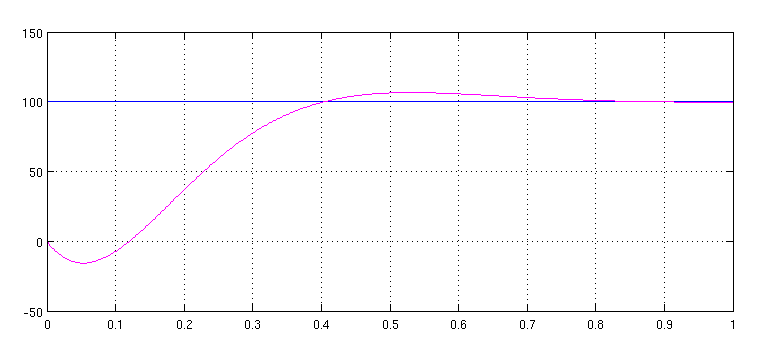
\includegraphics[scale=0.4]{simulation2.png}
	\caption{}
	\label{fig3}
\end{figure}
\noindent
La simulación del sistema muestra la siguiente respuesta a una entrada tipo escalón de amplitud $100$:
\begin{figure}[H]
	\centering
		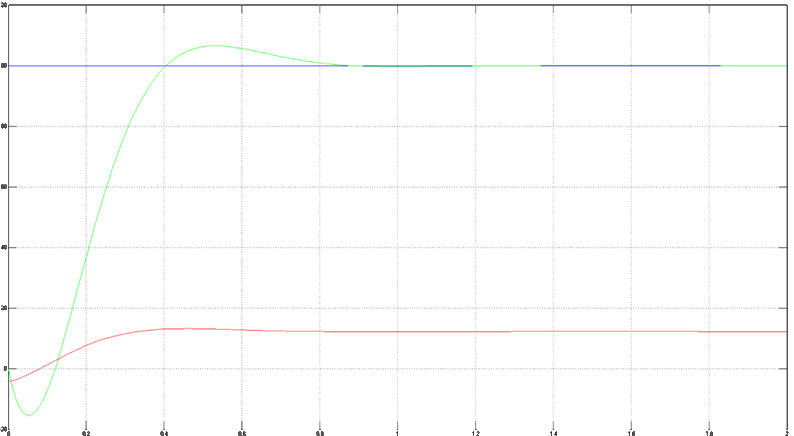
\includegraphics[scale=0.3]{simulation3.png}
	\caption{Respuesta  en simulación del sistema de control PI de motor LEGO}
	\label{fig5}
\end{figure}
\noindent
La respuesta del sistema cuenta con las especificaciones propuestas, mostrando un sobrepico de $6\%$, un tiempo de estabilización de aproximadamente $0.5$ segundos cuando donde la respuesta se encuentra dentro del rango del $5\%$ de su valor estacionario, y un error de posición cero. Se observa que al comienzo de la respuesta existe un periodo de tiempo donde se genera una respuesta negativa, este comportamiento es proporcionado por el cero del numerador que se encuentra en el semiplano derecho, lo que genera el subpico (undershoot).\\
La implementación experimental por medio del Brick NXT  frente a una entrada paso de $600\ \ rad/s$, muestra los siguientes resultados:
\begin{figure}[H]
	\centering
		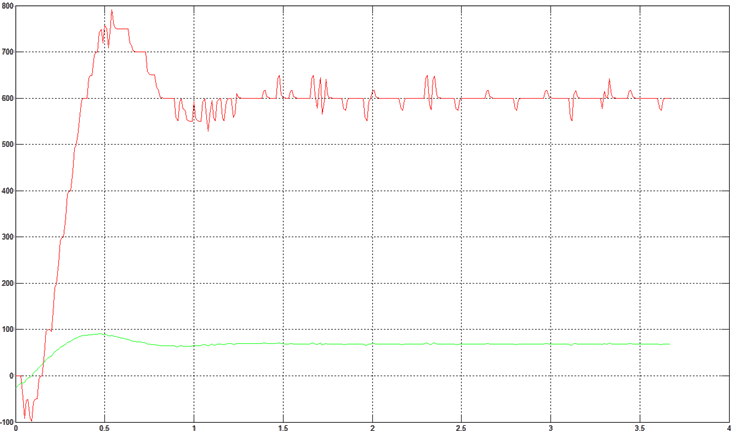
\includegraphics[scale=0.35]{salida2.png}
	\caption{Experimentales del control PI del motor LEGO}
	\label{fig6}
\end{figure}
\noindent
La implementación real del sistema de control muestra un comportamiento similar al obtenido en la simulación, con error permanente de posición cero y la acción del cero en la dinámica del sistema. 

\subsubsection{Punto 4.2.3}
\noindent
En este método se busca es cancelar un polo, y el sistema responderá como un sistema de primer orden.\\
Para ello se hace lo siguiente:
\begin{equation}
 G_{LC} \left( s \right) = \frac{{G_c \left( s \right)G_p \left( s \right)}}{{1 + G_c \left( s \right)G_p \left( s \right)}}
\label{ecu104}
\end{equation}
\noindent
Donde $G_c(s)$ es la función de transferencia del controlador y $G_p(s)$ es la función de transferencia de la planta.\\
Para la función de transferencia $G_{LC}(s)$ se tiene que reemplazando $G_p(s)=\frac{K_p}{\tau s + 1}$ y $G_{LC}(s)=K_c \left( {1 + \frac{1}{{T_i s}}} \right)$
\begin{equation}
 G_{LC} \left( s \right) = \frac{{K_c \left( {1 + \frac{1}{{T_i s}}} \right)\frac{{K_p }}{{\tau s + 1}}}}{{1 + K_c \left( {1 + \frac{1}{{T_i s}}} \right)\frac{{K_p }}{{\tau s + 1}}}}
\label{ecu105}
\end{equation}
\begin{equation}
 G_{LC} \left( s \right) = \frac{{K_c \left( {\frac{{1 + T_i s}}{{T_i s}}} \right)\frac{{K_p }}{{\tau s + 1}}}}{{1 + K_c \left( {\frac{{1 + T_i s}}{{T_i s}}} \right)\frac{{K_p }}{{\tau s + 1}}}}
\label{ecu106}
\end{equation}
\noindent
Dada la ecuación anterior si se hace $T_i=\tau$, se obtiene
\begin{equation}
 G_{LC} \left( s \right) = \frac{{K_c K_p \left( {1 + \tau s} \right)}}{{\tau s\left( {1 + \tau s} \right) + K_c K_p \left( {1 + \tau s} \right)}}
\label{ecu107}
\end{equation}
\noindent
La función de transferencia final de lazo cerrado quedaría
\begin{equation}
 G_{LC} \left( s \right) = \frac{1}{{\frac{\tau }{{K_c K_p }}s + 1}}
\label{ecu108}
\end{equation}
\noindent
Donde el nuevo $\tau '=\frac{\tau }{K_c K_p }$, entonces $K_c = 0.066$ y $T_i = 0.054$.\\
\begin{figure}[H]
	\centering
		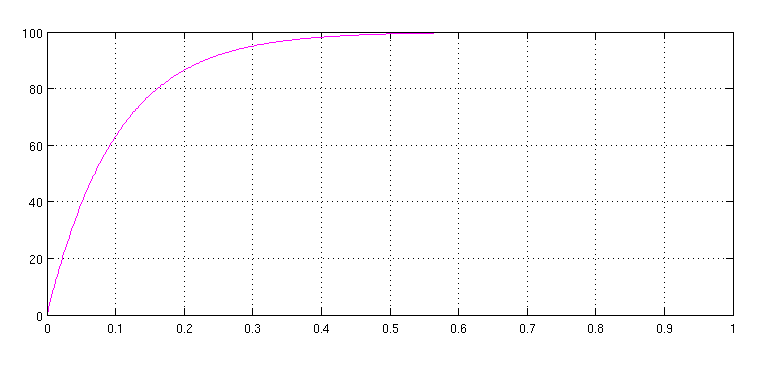
\includegraphics[scale=0.4]{salida32.png}
	\caption{Simulación Cancelación Polo-Cero}
	\label{fig6}
\end{figure}
\begin{figure}[H]
	\centering
		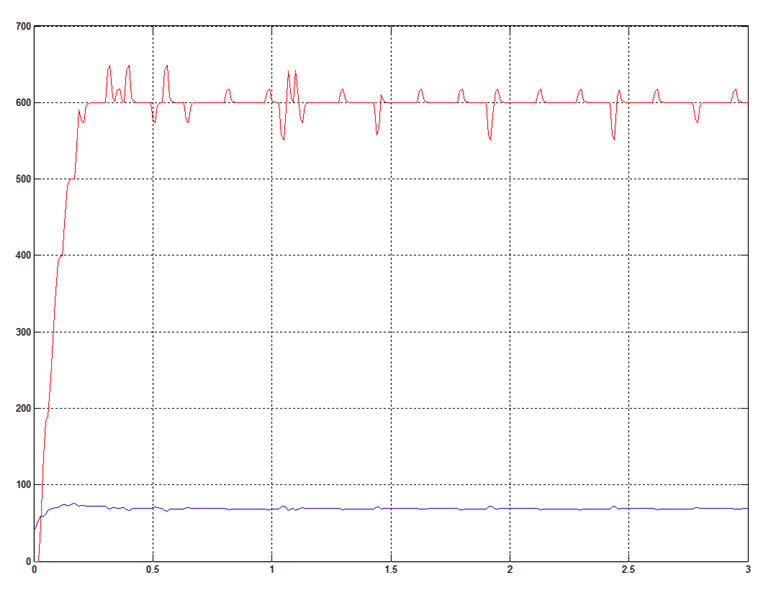
\includegraphics[scale=0.3]{practica3.png}
	\caption{Resultado Cancelación Polo-Cero}
	\label{fig6}
\end{figure}
\noindent
La implementación real del sistema de control muestra un comportamiento similar al obtenido en la simulación, con error permanente de posición cero y la acción del cero en la dinámica del sistema.

\subsubsection{Punto 4.2.4}
\noindent
Se busca hallar el valor de ganancia proporcional $K_p$ para un sistema de control de posición del motor LEGO, por medio de la técnica del lugar geométrico de las raíces, tal que la respuesta en lazo cerrado del sistema ante una entrada tipo escalón presente un sobrenivel porcentual del $35\%$.\\
La función de transferencia en lazo cerrado es la siguiente
\begin{equation}
 G\left( s \right) = \frac{{8.181818K_p }}{{0.054s^2  + s + 8.181818}} = \frac{{151.5151K_p }}{{s^2  + 18.5185s + 151.5151K_p }}
\label{ecu8}
\end{equation}
\noindent
Para desarrollar la técnica del lugar geométrico de las raíces es necesario tomar la función de transferencia en lazo abierto para determinar la condición de magnitud
\begin{equation}
 \left| {G_{LC} \left( s \right)} \right| = \left| {\frac{{8.181818K_p }}{{s\left( {0.054s + 1} \right)}}} \right| = 1
\label{ecu9}
\end{equation}
\noindent
Siendo el ángulo $\beta$ el ángulo entre la parte real y la parte imaginaria de los polos complejos del sistema de segundo orden, se realiza el siguiente análisis:
\begin{equation}
 \zeta  = \frac{{\left| {\ln \left( {0.35} \right)} \right|}}{{\sqrt {\left| {\ln ^2 \left( {0.35} \right)} \right| + \pi ^2 } }} \cong 0.316941
\label{ecu10}
\end{equation}
\begin{equation}
 \beta  = \cos ^{ - 1} \left( \zeta  \right) = 1.24829\ \ rad = 71.522^\circ 
\label{ecu11}
\end{equation}
\noindent
El número de asíntotas en el plano complejo son:
\begin{equation}
 \# A_s = n_p  - n_z  = 2 - 0 = 0
\label{ecu12}
\end{equation}
\noindent
Siendo $n_p$ el número de polos y $n_z$ el número de ceros. La magnitud de la parte real de los polos conjugados se halla a partir de la siguiente ecuación:
\begin{equation}
 \sigma  = \frac{{\sum {Polos}  - \sum {Ceros} }}{{n_p  - n_z }} = \frac{{\left( {0 - 18.5185} \right) - 0}}{{2 - 0}} =  - 9.25926
\label{ecu13}
\end{equation}
\noindent
Conociendo la parte real y el angulo de los polos complejos se obtienen los siguientes polos complejos conjugados, que permiten obtener el máximo sobrepico deseado:
\begin{equation}
 S_1  =  - 9.25926 + 27.7084i,\ \ S_2  =  - 9.25926 - 27.7084i
\label{ecu14}
\end{equation}
\noindent
Aplicando la condición de magnitud se encuentra el valor de $K_p$, tomando cualquiera de los polos anteriores:
\begin{equation}
 K_p  = \frac{{\left| s \right|\left| {0.054s + 1} \right|}}{{8.181818}} = 5.63302
\label{ecu15}
\end{equation}
\noindent
El diseño en Simulink mostrado a continuación permite simular la dinámica del sistema y comprobar la solución encontrada:
\begin{figure}[H]
	\centering
		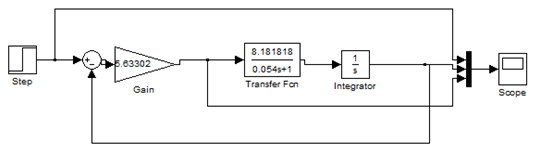
\includegraphics[scale=0.33]{diagram2.png}
	\caption{Diagrama en Simulink del sistema de control P de posición de motor LEGO}
	\label{fig7}
\end{figure}
\noindent
El resultado de la simulación muestra el siguiente comportamiento frente a una entrada paso de magnitud $100\ \ rad$:
\begin{figure}[H]
	\centering
		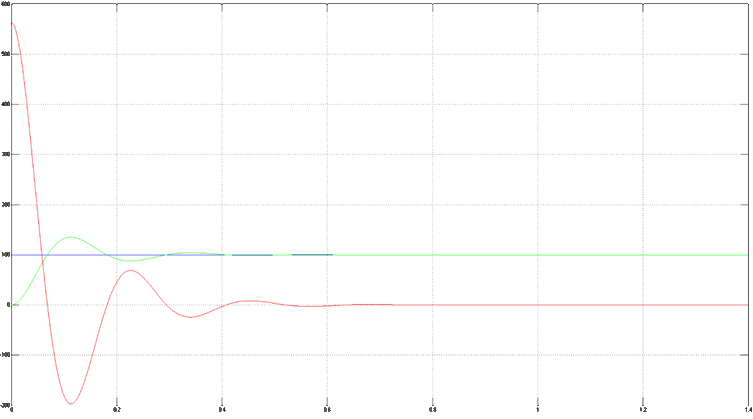
\includegraphics[scale=0.31]{salida3.png}
	\caption{Respuesta en simulación del sistema de control de posición del motor LEGO}
	\label{fig8}
\end{figure}
\noindent
Como se puede observar en la figura anterior, la respuesta del sistema alcanza el sobrepico en aproximadamente $135\ \ rad$, antes de estabilizarse con un error permanente de posición cero, por lo que el Kp calculado permite llegar a los resultados buscados idealmente. La señal de control como se muestra en la figura, tiene valores que en la implementación real producen la saturación del NXT llegando a un máximo de $100$ y un mínimo de $-100$, por lo que un diseño de simulación más apropiado se muestra a continuación:
\begin{figure}[H]
	\centering
		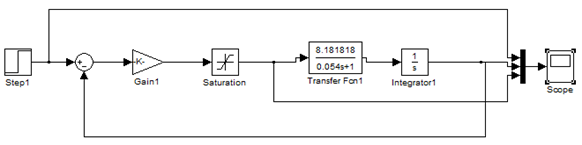
\includegraphics[scale=0.35]{tf32.png}
	\caption{Diagrama en Simulink del sistema de control P de posición de motor LEGO con saturación}
	\label{fig9}
\end{figure}
\noindent
El resultado de la simulación del diseño anterior es:
\begin{figure}[H]
	\centering
		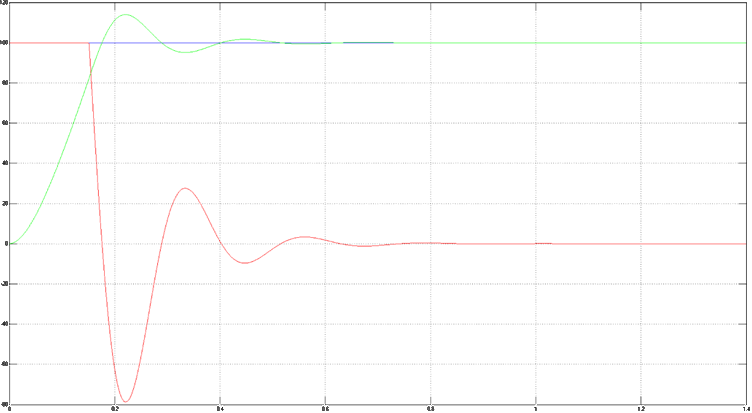
\includegraphics[scale=0.33]{salida4.png}
	\caption{Respuesta en simulación del sistema de control de posición del motor LEGO con saturación}
	\label{fig10}
\end{figure}
\noindent
Esta respuesta es más aproximada a la que se obtiene mediante la implementación real, debido a que cuenta con la limitación del Brick respecto a los valores que puede tomar la señal de control. Esto produce que la señal se demore más es en llegar al valor estacionario, pero disminuye el máximo sobrepico.\\
La realización de la prueba del sistema de control con la ganancia $K_p$ encontrada muestra el siguiente resultado:
\begin{figure}[H]
	\centering
		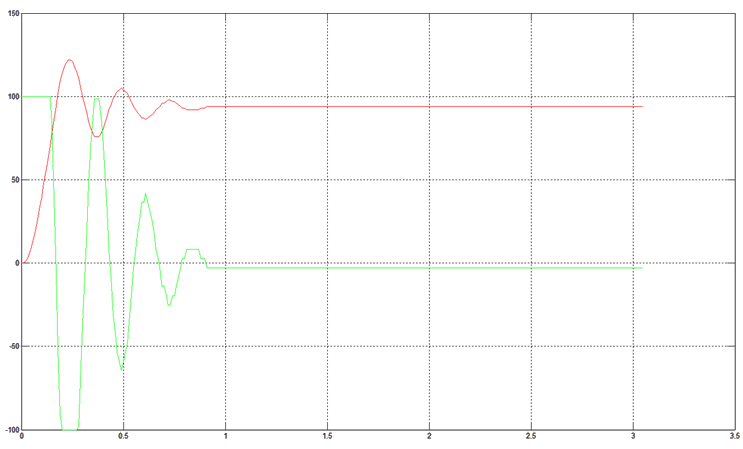
\includegraphics[scale=0.33]{salida5.png}
	\caption{Resultados Experimentales del control de posición del motor LEGO}
	\label{fig11}
\end{figure}
\noindent
Los resultados experimentales presentan más oscilación y un error permanente en estado estacionario, debido a la fricción que se genera en el motor y la cantidad de energía que el controlador le entrega al motor. El máximo sobre pico se encuentra en un $22\%$ y el tiempo de estabilización es similar al obtenido en la simulación. El error generado por la fricción puede ser resulto por medio de un control integral que acumule el error  generado y realice una acción de control correctiva.

\subsubsection{Punto 4.2.5}
\noindent
Para este diseño se implemento un PD, dado que un PI aumenta el grado del denominador de la función de transferencia en lazo cerrado, y un P no es suficiente para obtener un error de estado estacionario en 0.\\
Se utilizo el diagrama de funcionamiento del BricxCC, el cual es
\begin{figure}[H]
	\centering
		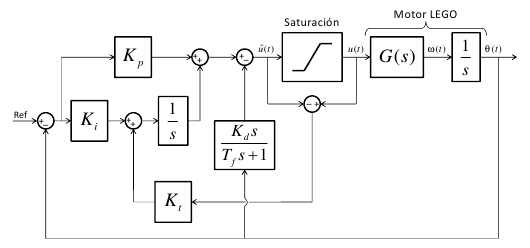
\includegraphics[scale=0.65]{bricx.png}
	\caption{ Estructura del sistema de control de posición implementado en \textit{controlPIDpos.nxc}.}
	\label{fig11}
\end{figure}
\noindent
Al hacer cero el valor de $K_i$, $K_t$ y $T_f$ se obtiene la siguiente función de transferencia
\begin{equation}
 G_{LC} \left( s \right) = \frac{{KK_p }}{{s\left( {\tau s + 1} \right) + KK_d s + KK_p }}
\label{ecu109}
\end{equation}
\begin{equation}
 G_{LC} \left( s \right) = \frac{{\frac{{KK_p }}{\tau }}}{{s^2  + s\left( {\frac{{1 + KK_d }}{\tau }} \right) + \frac{{KK_p }}{\tau }}}
\label{ecu110}
\end{equation}
\noindent
Donde $K$ es la ganancia de la planta y $\tau$ es el tiempo de respuesta de la planta. Dado que se necesita un sobre nivel porcentual inferior al $7\%$ y un tiempo de estabilización igual a $0.2seg$, y utilizando las ecu. (\ref{ecu5}) y ecu. (\ref{ecu4}). Se obtiene que
\begin{equation}
 2\zeta \omega _n  = \frac{{K K_d  + 1}}{\tau } ;\ \ \omega _n ^2  = \frac{{K K_d }}{{T_i \tau }}
\label{ecu111}
\end{equation}
\noindent
Al realizar el despeje adecuado se obtienen los siguientes resultados
\begin{equation}
 K_d = 0.075777\ \ y\ \ K_p = 3.3366
\label{ecu112}
\end{equation}
\begin{figure}[H]
	\centering
		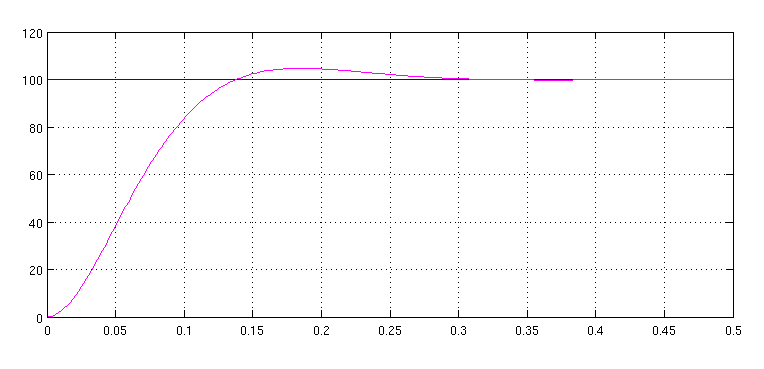
\includegraphics[scale=0.43]{practica4.png}
	\caption{Simulación obtenida del controlador PD.}
	\label{fig15}
\end{figure}
\begin{figure}[H]
	\centering
		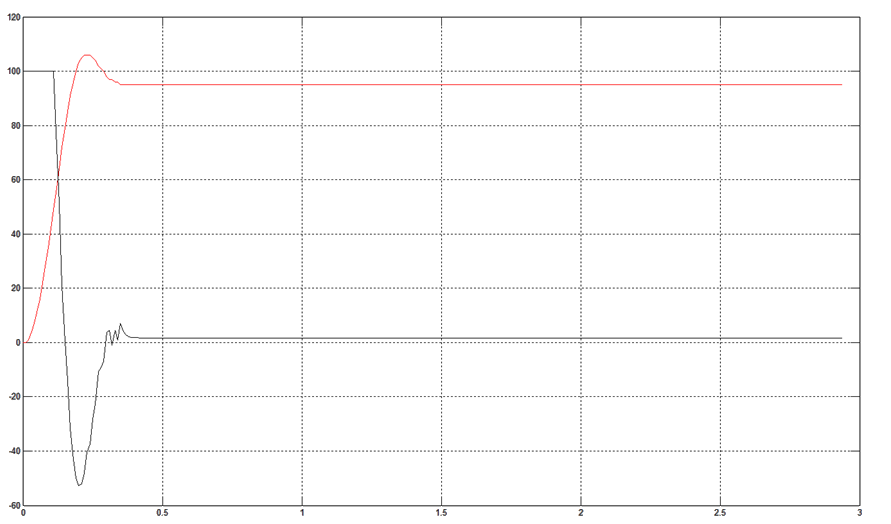
\includegraphics[scale=0.27]{ultima.png}
	\caption{Salida obtenida del controlador y respuesta.}
	\label{fig20}
\end{figure}
\noindent
El error de estado estacionario que se observa en la gráfica es debido a la fricción que se encuentra en el motor dado que solo tiene una parte proporcional y una parte derivativa, pero en la simulación dicho error es cero. Es necesario saber que tipo de controlador se va a implementar en dicha planta, como se dijo al principio de este inciso se intento con un controlador P y no fue suficiente, dado que tenia error constante. Y un PI nos aumentaba en un grado el numerador de la función de transferencia en lazo cerrado. Por ello se diseño con un PD.

\section{Conclusiones}
\begin{itemize}
 \item En este laboratorio se ha comparado diferentes métodos de sintonización de controladores, cada uno tiene sus ventajas y desventajas, el uso de uno u otro método o criterio  depende siempre del proceso que se vaya a controlar, pues este nos dirá si es aceptable o no un sobrepico o un tiempo de respuesta lento, etc.
 \item La optimización de un controlador PID esta en escoger los mejores valores para sus parámetros ($K_c$, $T_i$ ,$T_d$). Logrando a través de esto una respuesta rápida sin altos sobrepicos y con un error de estado estacionario mínimo.
 \item El método de modelado por tiempo muerto y  respuesta de primer orden es una herramienta  muy útil a la hora de analizar diferentes sistemas ya que simplifica mucho el análisis de procesos cuya respuesta esta caracterizada por sistemas de alto orden.
 \end{itemize}

\bibliographystyle{ieeetran}
\begin{thebibliography}{99}

\bibitem{chen} Chen, Chi-Tsong.
{\em "`Analog and Digital Control System Desing: Transfer-Function, State, Space and Algebraic Methods"'}.
Saunders College Publishing, 1993.

\bibitem{kuo} Kuo, C. Benjamin.
{\em "`Sistemas Automáticos de Control"'}.
Pentice Hall Hispanoamerica, Séptima Edición, 1996.

\bibitem{ogata} Ogata, Katsuhiko.
{\em "`Ingeniería De Control Moderna"'}.
Pearson Educación, Tercera Edición, 1998.

\end{thebibliography}
\end{document}